%% Exemplo de utilizacao do estilo de formatacao normas-utf-tex (http://normas-utf-tex.sourceforge.net)
%% Autores: Hugo Vieira Neto (hvieir@utfpr.edu.br)
%%          Diogo Rosa Kuiaski (diogo.kuiaski@gmail.com)
%% Colaboradores:
%%          Cézar M. Vargas Benitez <cesarvargasb@gmail.com>
%%          Marcos Talau <talau@users.sourceforge.net>


\documentclass[openright]{normas-utf-tex} %openright = o capitulo comeca sempre em paginas impares
%\documentclass[oneside]{normas-utf-tex} %oneside = para dissertacoes com numero de paginas menor que 100 (apenas frente da folha) 


\usepackage[alf,abnt-emphasize=bf,bibjustif,recuo=0cm, abnt-etal-cite=2, abnt-etal-list=99]{abntcite} %configuracao correta das referencias bibliograficas.

\usepackage[brazil]{babel} % pacote portugues brasileiro
\usepackage[utf8]{inputenc} % pacote para acentuacao direta
\usepackage{amsmath,amsfonts,amssymb} % pacote matematico
\usepackage{graphicx} % pacote grafico
\usepackage{times} % fonte times
\usepackage{listings} % para código-fonte
\usepackage{algorithmic}

% configuracao do pacote listings
\lstset{
	basicstyle=\footnotesize,
	showstringspaces=false,
	tabsize=4,
	numbers=left,
	numberstyle=\tiny,
	stepnumber=1,
	numbersep=5pt,
	breaklines=true,
	extendedchars=true,
	frame=tb
}

%Podem utilizar GEOMETRY{...} para realizar pequenos ajustes das margens. Onde, left=esquerda, right=direita, top=superior, bottom=inferior. P.ex.:
%\geometry{left=3.0cm,right=1.5cm,top=4cm,bottom=1cm} 

% ---------- Preambulo ----------
\instituicao{Universidade Tecnol\'ogica Federal do Paran\'a} % nome da instituicao
\departamento{Departamento Acadêmico de Informática}
\programa{Curso Superior de Engenharia de Computação} % nome do programa

\documento{Proposta de Trabalho de Conclusão de Curso} % [Disserta\c{c}\~ao] ou [Tese]
\nivel{Graduação} % [Mestrado] ou [Doutorado]
\titulacao{Engenheiro} % [Mestre] ou [Doutor]

\titulo{\MakeUppercase{Degradação de Vídeos para Avaliação Subjetiva de Vídeo Digital}} % titulo do trabalho em portugues

\autor{Brunno Alberto Wistuba Braga} % autor do trabalho
\autordois{Caio Nogara Andreatta}
\cita{BRAGA, Brunno A. W.; ANDREATTA, Caio N.} % sobrenome (maiusculas), nome do autor do trabalho

\comentario{\UTFPRdocumentodata\ de graduação, apresentado à disciplina de Trabalho de Conclusão de Curso II, do \UTFPRprogramadata\ do \UTFPRdepartamentodata\ da \ABNTinstituicaodata\, como requisito parcial para obten\c{c}\~ao do grau de \UTFPRtitulacaodata.}



\orientador{Profª. Drª. Keiko Veronica Ono Fonseca} % nome do orientador do trabalho
%\orientador[Orientadora:]{Nome da Orientadora} % <- no caso de orientadora, usar esta sintaxe
%\coorientador{Nome do Co-orientador} % nome do co-orientador do trabalho, caso exista
%\coorientador[Co-orientadora:]{Nome da Co-orientadora} % <- no caso de co-orientadora, usar esta sintaxe
%\coorientador[Co-orientadores:]{Nome do Co-orientador} % no caso de 2 co-orientadores, usar esta sintaxe
%\coorientadorb{Nome do Co-orientador 2}	% este comando inclui o nome do 2o co-orientador

\local{Curitiba} % cidade
\data{\the\year} % ano automatico


%---------- Inicio do Documento ----------
\begin{document}

\capa % geracao automatica da capa
\folhaderosto % geracao automatica da folha de rosto
%\termodeaprovacao % <- ainda a ser implementado corretamente

% listas (opcionais, mas recomenda-se a partir de 5 elementos)
\listadefiguras % geracao automatica da lista de figuras
\listadetabelas % geracao automatica da lista de tabelas
\listadesiglas % geracao automatica da lista de siglas

% sumario
\sumario % geracao automatica do sumario


%---------- Inicio do Texto ----------
% recomenda-se a escrita de cada capitulo em um arquivo texto separado (exemplo: intro.tex, fund.tex, exper.tex, concl.tex, etc.) e a posterior inclusao dos mesmos no mestre do documento utilizando o comando \input{}, da seguinte forma:

% aparentemente esse sloppy resolve o problema das margens e do texttt
% não tenho certeza sobre os efeitos colaterais dele, no entanto
% fiquemos atentos! :P
\sloppy

\chapter{Introdução}

Contando com os avanços tecnológicos das últimas décadas, o vídeo digital se encontra cada vez mais presente no dia a dia das pessoas ao redor do mundo, seja como educação, entretenimento ou informação.
Além de acessível, também é necessário que o vídeo chegue a essas pessoas com um nível de qualidade que as possibilitem contemplar e interpretar as imagens de forma natural, sem exasperação do (\sigla{SVH}{Sistema Visual Humano}, ou seja, sem que existam perdas ou distorções exageradas em seu conteúdo.
No entanto, processos como aquisição, compressão, armazenamento e transmissão, os quais viabilizam e popularizam a difusão de vídeo, são muitas vezes responsáveis por também introduzir artefados que degradam a qualidade final da imagem \cite{daronco}.

No intuito de melhor avaliar o efeito que tais artefatos podem produzir no SVH foram desenvolvidas métricas objetivas e subjetivas de avaliação de qualidade de vídeo. O projeto SASQV, desenvolvido por \cite{sasqv}, busca implementar ambas as formas de avaliação em um mesmo conjunto de \emph{software} e \emph{hardware} onde é possível gerar artefatos articiais, coletar avaliações subjetivas e aplicar métricas objetivas sobre uma base de vídeos, também oferencendo ferramentas para análise e comparação dos dados obtidos. O presente trabalho propõe adaptações ao SASQV, buscando aperfeiçoar a ferramenta de  geração de artefatos no sentido de torna-los mais similares àqueles encontrados nas trasmissões, fornecendo maior grau de liberdade para a manipulação dos mesmos, além de agregar novos tipos, como por exemplo a simulação de um \emph{streaming} de vídeo. Dada a natureza do projeto SASQV, o qual se utiliza de softwares e bibliotecas distribuidos sob licenças de \emph{software} livre, este projeto também se propõe a construir uma nova interface gráfica não baseada em tecnologias proprietárias.

A proposta é motivada pela ampla difusão de vídeo digital, implantadas principalmente na forma de TV digital e de \emph{streaming} via internet, sendo o segundo objeto de grande interesse no mercado. Segundo \cite{sandvinereport}, no continente norte-americano cerca de 37\% do tráfego de internet fixa é dedicado ao \emph{streaming} de vídeo durante o horário onde tradicionalmente ocorre o pico de audiência televisiva, atingindo 41\% no caso da internet móvel dentro do mesmo horário.

\section{Palavras-Chave}
Vídeo digital, Geração de artefatos de vídeo digital, Avaliação subjetiva e objetiva de qualidade de vídeo.
\section{Objetivo Geral}
Adaptar a ferramenta \sigla{SASQV}{Sistema de Avaliação Subjetiva de Qualidade de Vídeo} no sentido de aprimorar a degradação, reprodução, manipulação, interação e portabilidade  presentes na ferramenta original.
\section{Objetivos Específicos}
\begin{itemize}
	\item \textbf{} Aprimorar os algoritmos de geração de artefatos (\emph{blocking} e \emph{blurring} - blocagem e embarassamento) de vídeo digital, permitindo ao usuário manipular os parâmetros de cada artefato.
	\item \textbf{} Adaptar a ferramenta original para manipular vídeo bruto no formato \emph{.yuv}.
	\item \textbf{} Adicionar à ferramenta um simulador de transmissões de vídeo via rede por meio de \emph{streaming} e seus possíveis artefatos.
	\item \textbf{} Desenvolver uma nova interface gráfica em linguagem Java.
	\item \textbf{} Aprimorar a portabilidade da ferramenta para sistemas operacionais diversos.
\end{itemize}


\chapter{Recursos de \emph{Hardware} e \emph{Software}}

\section{Recursos de \emph{Hardware}}

Este projeto não visa desenvolver ou aprimorar equipamentos físicos existentes no SASQV, portanto os recursos de \emph{hardware} permanecem inalterados em relação ao projeto de \cite{sasqv}. Como principais recursos podemos destacar o conjunto de dispositivos de entrada provido de comunicação sem fio, um dispositivo receptor capaz de se comunicar com os dispositivos de entrada e também um computador possuindo atributos de processamento e armazenamento capazes de receber um sistema gerenciador de banco de dados e suprir os requisitos necessários para reprodução de vídeo digital em qualidade \sigla{HD}{High Definition}.

\section{Recursos de \emph{Software}}

Sendo este continuidade do sistema SASQV, as tecnologias Java e MySQL serão utilizadas no projeto, assim como o \sigla{IDE}{Integrated Development Environment} Eclipse. Novidades serão introduzidas a partir da utilização da linguagem de programação C++ para construção de ferramentas auxiliares para manipulação dos vídeos. O projeto também terá versionamento de código e documentos, os quais se encontrarão disponíveis no repositório colaborativo github \cite{githubabout} e sendo gerenciado pela ferramenta livre git. 


%----------- Terceiro Capítulo: Metodologia --------------

\chapter{Especificação} %(ou especifiação) 10 --- 20 pags

O \emph{software} a ser desenvolvido neste trabalho deverá fornecer uma ferramenta flexível de degradação de vídeo digital e também de avaliação subjetiva e objetiva das mídias.
Neste capítulo serão apresentados os requisitos de tal sistema, assim como as especificações de desenvolvimento, arquitetura e funcionamento.

\section{Análise de Requisitos}

A análise de requisitos é parte fundamental de qualquer projeto, buscando atender da melhor forma as necessidades dos futuros usuários.
Esta sessão descreve os requisitos levantados durante o estudo e planejamento da ferramenta.

\subsection{Requisitos Funcionais}

Requisitos funcionais são aqueles determinados pelas funcionalidades exigidas do sistema, ou seja, as ações que se espera que o sistema execute. 
Foram levantados os seguintes requisitos funcionais:

\begin{itemize}
	\item O \emph{software} deverá possuir ferramentas de degradação de vídeos digitais de blocagem e borramento.
	\item O \emph{software} deverá possuir uma ferramenta de simulação de transmissão \emph{streaming}.
	\item O \emph{software} deverá ser capaz de criar e gerenciar sessões de avaliação subjetiva.
	\item O \emph{software} deverá possuir uma ferramenta que realize avaliação objetiva sobre os vídeos da base de dados, conforme as métricas PSNR, MSE e MSSIM.
	\item O \emph{software} deverá ser capaz de exibir os vídeos existentes na base de dados.
	\item O \emph{software} deverá exibir os resultados das avaliações objetivas e subjetivas de forma gráfica.
\end{itemize}

\subsection{Requisitos Não-Funcionais}

Requisitos não-funcionais são aqueles ditados por restrições ou exigências de qualidade ou de operação, tais como performance, segurança ou tecnologias envolvidas.
Abaixo se encontram os requisitos não funcionais levantados:

% TODO dividir por categorias: padronização, usabilidade, tecnologias envolvidas.

\begin{itemize}
	\item As ferramentas de degradação e métricas objetivas deverão operar sobre vídeos em formato YUV planificado com subamostragem 4:2:0.
	\item A ferramenta de simulação deverá operar sobre vídeos no formato \sigla{H.262}{Padrão de compressão de vídeo digital também conhecido MPEG-2 Part 2} encapsulados em um Transport Stream (\sigla{TS}{Transport Stream}).
	\item O sistema deve fornecer documentação detalhada de auxílio ao uso das ferramentas.
	\item A ferramenta de exibição deverá ser executada em um sistema capaz de prover um \emph{display} com resolução igual ou maior que a dos vídeos a serem exibidos.
	% TODO verificar a versão da JRE necessária para rodar a interface
	\item A interface gráfica do sistema necessita que haja um \emph{Java Runtime Environment} (\sigla{JRE}{Java Runtime Environment}) instalado no sistema operacional.
	\item O \emph{player} de vídeo MPlayer, livre e de código aberto, é necessário para mostrar os vídeos durante as sessões.
\end{itemize}

\section{Especificações do Software}

Esta seção tem o propósito de descrever a arquitetura proposta para o SASQV2, assim como abordar as diferentes linguagens e bibliotecas que ajudam a integrar o programa.

\subsection{Arquitetura do Sistema}

Por se tratar da continuação do desenvolvimento do projeto SASQV, este trabalho reutiliza e adapta grande parte dos componentes existentes no trabalho original.

A Figura \ref{fig:arquitetura} mostra uma comparação entre as visões gerais de ambos os projetos. A diferença mais notável entre estas arquiteturas é a separação dos componentes de serviço e o de ferramentas, além de também recriar o componente de interface gráfica para melhor atender às necessidades do sistema.

Mais detalhes sobre cada componente da arquitetura são descritos em seções específicas a seguir.

\begin{figure}[!htb]
	\centering
	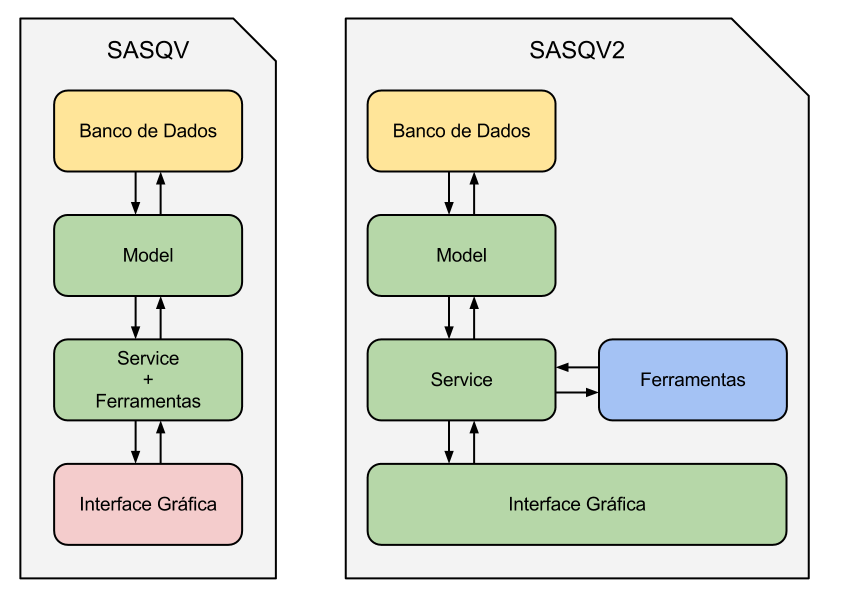
\includegraphics[width=0.9\textwidth]{./imgs/arquitetura.png}
	\caption{Visão geral das arquiteturas dos sistemas SASQV e SASQV2.}
	\label{fig:arquitetura}
	\fonte{Autoria Própria.}
\end{figure}

\subsubsection{Banco de Dados}

O componente banco de dados foi completamente reaproveitado, seguindo as mesma especificações do SASQV.

O Sistema Gerenciador de Banco de Dados (\sigla{SGBD}{Sistema Gerenciador de Banco de Dados}) escolhido foi o MySQL, atualmente o SGDB \emph{open source} mais utilizado no mundo \cite{mysqlmarket}.
O MySQL foi lançado e desenvolvido em 1995 pela empresa Sueca MySQL AB, atualmente incorporada pela Oracle Corporation, na forma de um SGDB que fornece um servidor multi-usuários para bancos de dados relacionais \cite{wikipediamysql}.

Juntamente do MySQL também é utilizado o MySQL Workbench, uma ferramenta distribuída pela Oracle que concilia um cliente MySQL, uma ferramenta de \emph{Database Moddeling} e um administrador de servidor MySQL.

A versão \emph{open source} de ambas as ferramentas é distribuída sob a licensa GNU General Public License (\sigla{GPL}{General Public License}).

O modelo Entidade-Relacionamento (\sigla{ER}{Entidade-Relacionamento}) é o mesmo utilizado pelo SASQV, como mostrado na Figura \ref{fig:diagramaER}.

\begin{figure}[!htb]
	\centering
	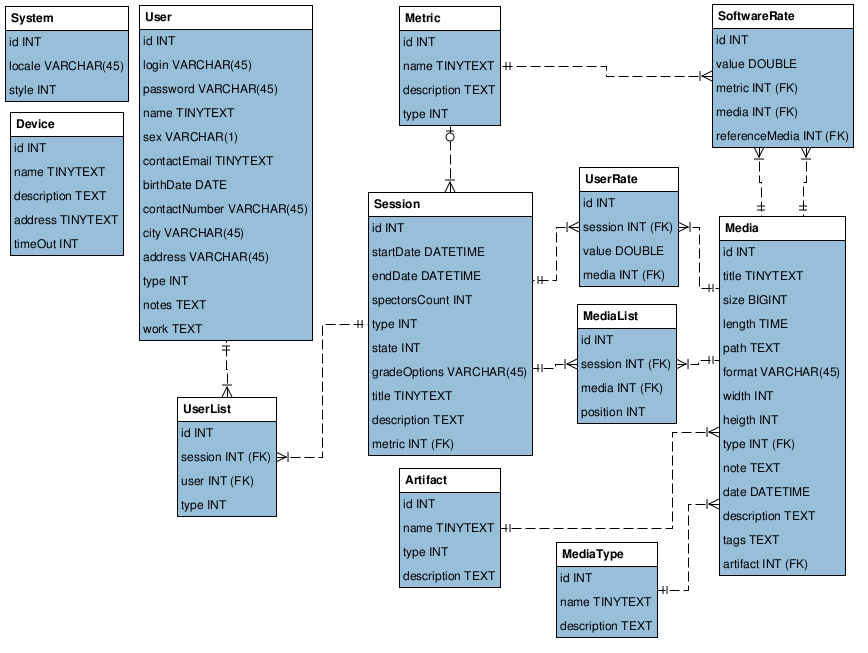
\includegraphics[width=0.9\textwidth]{./imgs/diagramaER.png}
	\caption{Diagrama Entidade-Relacionamento do SASQV2}
	\label{fig:diagramaER}
	\fonte{Autoria Própria}
\end{figure}

\subsubsection{Model}

O componente Model presente no SASQV2 também foi inteiramente reaproveitado do SASQV, cabendo apenas algumas adições. Este componente consiste na implementação de um mapeamento objeto-relacional (\sigla{MOR}{Mapeamento Objeto Relacional}) por meio da biblioteca Hibernate.

O Hibernate teve seu desenvolvimento iniciado em 2001 por Gavin King, com o objetivo de melhorar as ferramentas de persistência existentes na plataforma Java \cite{hibernateHistory}, e é atualmente distribuído sob a licensa GNU Lesser General Public License (\sigla{LGPL}{Lesser General Public License}) \cite{hibernateAbout}.

A biblioteca provê um mapeamento flexível entre objetos Java e tipos SQL, eliminando a custosa necessidade de processamento manual e repetitivo de listas de resultados obtidas via SQL e JDBC.
Estima-se que até cerca de 30\% do código de uma aplicação possa ser poupado utilizando MOR, além de incrementar a portabilidade do sistema suportando diversas implementações de Bancos de Dados SQL em troca de um pequeno \emph{overhead} de performance.

\subsubsection{Service}

Este elemento também foi reaproveitado, no entanto sofreu diversas adaptações em sua estrutura para comportar novas funcionalidades e continuar suportando as antigas.
O componente presente no SASQV se trata de uma fachada de serviço responsável por interpretar mensagens provenientes da interface e distribuí-las em uma das três formas a seguir:

\begin{enumerate}
	\item Executar uma ação de degradação ou métrica objetiva.
	\item Repassar uma ação para o dispositivo sem-fio e esperar por resposta.
	\item Repassar uma ação para o elemento model e esperar por resposta.
\end{enumerate}

Na arquitetura do SASQV2 a interpretação de mensagens foi descartada, uma vez que foi prosposta a implementação de uma nova interface em linguagem Java, que deu lugar a métodos de finalidades distintas dentro de cada ação enumerada acima. % TODO verificar se o acima pode virar abaixo?!!?
Com isso a execução de tarefas de degradação ou avaliação por métrica objetiva, antes executadas localmente, passaram a ser delegadas para um novo componente chamado Ferramentas, descrito em \ref{met:ferramentas}.

Já o conteúdo dos métodos que repassam as ações para o dispositivo sem-fio e para o model permanecem muito semelhantes aos encontrados na interpretação de mensagens originalmente feito no SASQV, sofrendo apenas pequenas modificações para acomodar a nova estrutura.

\subsubsection{Ferramentas}
\label{met:ferramentas}

O módulo ferramentas constitui um novo componente na arquitetura do \emph{software}, visto que um dos objetivos deste trabalho é desenvolver melhores ferramentas de degradação considerou-se válida a separação deste módulo que originalmente se encontrava juntamente do Service.

Esse módulo é resposável por todas as ferramentas que de alguma forma manipulam vídeos digitais ou auxilíam nesta manipulação. Dessa forma foram desenvolvidas 5 ferramentas distintas, em linguagem C++:

\begin{description}
	\item[Block] Cria o efeito de blocagem nos vídeos.
	\item[Blur] Cria o efeito de embaçamento nos vídeos.
	\item[Netsim] Efetua uma simulação de streaming de vídeo digital com perda informação.
	\item[Raffle] Ferramenta auxíliar para distribuição temporal e espacial dos artefatos.
	\item[Metric] Efetua avaliação dos vídeos por meio de métricas objetivas.
\end{description}

Estas ferramentas podem receber configurações independentes e flexíveis, diversificando as possibilidades de geração de degradações e artefatos e tornando possível a criação de resultados diferenciados para um mesmo vídeo usado como referência. Dentre essas configurações pode-se destacar a distribuição dos artefatos no tempo e no espaço e a intensidade de aplicação dos mesmos. Cada ferramenta citada será descrita com mais detalhes em \ref{des:ferramentas}. 

\subsubsection{Interface Gráfica}


Originalmente desenvolvida utilizando a tecnologia Adobe Flex, era necessária a utilização de uma biblioteca exclusivamente para comunicação entre os módulos de Interface e Service. A biblioteca utilizada (merapi) se encontrava em fase de desenvolvimento beta e carecia de funcionalidades, de forma que seria necessário buscar uma biblioteca alternativa para continuar o densevolvimento do projeto.

Além disso, as ferramentas de desenvolvimento em tecnologia Flex não são gratuitas e perderam gradativamente o suporte à sistemas operacionais Linux.

A combinação destes fatores motivou a decisão de desenvolver uma nova intercae Gráfica utilizando Java, proporcionando melhor integração, reduzindo o envolvimento de diversas tecnologias e bibliotecas e assim aumentando a portabilidade da ferramenta.

\subsection{Linguagens}

Por se tratar da aprimoração e continuação do projeto SASQV a primeira linguagem contemplada foi a presente no mesmo: Java.

Esta foi desenvolvida por uma equipe de programadores liderada por James Gosling, trabalhando para a empresa Sun MicroSystems \cite{wikijava}. Sendo lançada em 1995, era o principal componente da plataforma Java e demonstrava forte inspiração na linguagem C++, compartilhando parte de sua sintaxe e também diversas característica.

No entanto, Java é considerada uma linguagem de mais alto nível, além de ser compilada no formato \emph{bytecode}, o que favorece a portabilidade dos programas, podendo ser executados em diversas arquiteturas e sistemas operacionais, contanto que estes possuam uma implementação da Java Virtual Machine (\sigla{JVM}{Java Virtual Machine}). Uma das facilidades da linguagem é a sua extensa biblioteca padrão, que contém, entre outros, diversos componentes para construção de interfaces gráficas.

A linguagem C++ também passou a ser considerada para o desenvolvimento do projeto, visto o desenvolvimento do módulo de Ferramentas como programas que possam ser usados independentemente.
A linguagem teve seu desenvolvimento iniciado por Bjarne Stroustrup em 1979, quando trabalhava na Bell Labs \cite{wikicplusplus}.
C++ é uma nova implementação da linguagem C adicionada de novas funcionalidades, tais como suporte a classes, sobrecarga de operadores, herança múltipla e tratamento de exceções.
Atualmente, C++ é uma das linguagens mais populares, sendo implementada em diversas plataformas de \emph{hardware} e sistemas operacionais, além de ser usada na implemantação dos mais diversos \emph{softwares} para \emph{desktop}, \emph{drivers} de dispositivos de \emph{hardware} e sistemas embarcados.

Um dos principais atrativos da linguagem para o desenvolvimento das ferramentas deste projeto é a existência de diversas funcionalidades de baixo nível.
Essas funcionalidades simplificam e facilitam o acesso e manipulação \emph{byte} a \emph{byte} de \emph{streams} de dados, algo que é usado extensivamente ao longo da implementação das ferramentas.
Outro aspecto importante derivado destas funcionalidades é o impacto na performance do software. 
Segundo \cite{benchmarks}, para o \emph{benchmark reverse-complement} --- onde são efetuadas diversas operações de leitura e escrita em arquivos, além de um leve processamento --- a melhor implementação em Java foi 1.9 vezes mais lenta que a melhor implementação em C++.
A simplicidade da linguagem também facilita o desenvolvimento de ferramentas \emph{stand-alone} com interface por linhas de comando, além de possuir diversas bibliotecas de \emph{parsing} para comandos e opções.

Ambas as linguagens eram previamente conhecidas pelos integrantes do projeto, os quais também possuem um nível confortável de experiência no desenvolvimento de aplicações com estas linguagems e com diversas ferramentas associadas a elas, como IDE's, bibliotecas gráficas e conectividade com bancos de dados.

\subsection{Bibliotecas}
\subsection{Diagramas de Caso de Uso}
\section{Considerações}

Para este projeto de \emph{software} procurou-se aproveitar ao máximo os componentes existentes no SASQV, de forma a maximizar o esforço nos aspectos a serem melhorados e não consumir tempo de projeto retrabalando o que já foi feito. 

A adesão ao desenho de \emph{software} apresentado se justifica pela independência entre os componentes, facilitando o desenvolvimento e teste de cada um e também o reaproveitamento em trabalhos futuros.
A opção por criar ferramentas independentes para o processo de degradação se mostra eficiente e versátil, visto que deste modo estão prontas para serem reutilizadas e combinadas à outras ferramentas, além de facilitarem a automatização do processo de degradação para o usuário avançado.

Sendo assim, a estrutura planejada foi muito semelhante à do projeto original, com diversos componentes sofrendo adaptações e também a adição de um novo componente dedicado.


\chapter{Contexto}


\section{Conclusão}

% ------ estrutura
\subsection{Conclusões}
    \begin{frame}\frametitle{Completude dos Objetivos}
	Quanto às ferramentas:
	\begin{itemize}
		\item Geradores de artefatos
		\begin{itemize}
			\item Configuráveis de forma flexível
			\item Oferecem mais opções
			\item Trabalham sobre arquivos YUV
		\end{itemize}
		\item{Arquivo de degradação}
		\begin{itemize}
			\item Permite reprodução e controle sobre os artefatos
			\item Economia de espaço
		\end{itemize}
		\item Simulador
		\begin{itemize}
			\item Dispensa interfaces físicas
			\item Configurações flexíveis
		\end{itemize}
	\end{itemize}
    \end{frame}

	\begin{frame}\frametitle{Completude dos Objetivos}
	Quanto à Interface:
	\begin{itemize}
		\item Funcionalidades semelhantes ao SASQV
		\item Adaptações para agregar ferramentas e novas utilidades
	\end{itemize}
	Quanto ao sistema:
	\begin{itemize}
		\item Portável, disponível em um arquivo \emph{.jar}
		\item Ferramentas independentes, disponíveis em C++
	\end{itemize}
	\end{frame}
    
\subsection{Trabalhos Futuros}
    \begin{frame}\frametitle{Sugestões}
	\begin{itemize}
		\item extender a funcionalidade do \emph{hardware}
		\item novas ferramentas independentes podem ser criadas
		\item adaptações no BD, agregando mais resultados
		\item aprimoramento da simulação
	\end{itemize}
    \end{frame}
    
\subsection{Fim}
    \begin{frame}\frametitle{Obrigado!}
        \begin{table}[!h]
	        \begin{tabular}{lll}
                Brunno Braga & 41-8898-4111 & brunnobga@gmail.com \\
                Caio Andreatta & 41-8448-7157 & caioccaa@gmail.com \\
	        \end{tabular}
        \end{table}
    \end{frame}



%---------- Referencias ----------
\bibliography{proposta} % geracao automatica das referencias a partir do arquivo reflatex.bib

%-------- Citacoes ---------
% - Utilize o comando \citeonline{...} para citacoes com o seguinte formato: Autor et al. (2011).
% Este tipo de formato eh utilizado no comeco do paragrafo. P.ex.: \citeonline{autor2011}

% - Utilize o comando \cite{...} para citacoeses no meio ou final do paragrafo. P.ex.: \cite{autor2011}



%-------- Titulos com nomes cientificos (titulo, capitulos e secoes) ----------
% Regra para escrita de nomes cientificos:
% Os nomes devem ser escritos em italico, 
%a primeira letra do primeiro nome deve ser em maiusculo e o restante em minusculo (inclusive a primeira letra do segundo nome).
% VEJA os exemplos abaixo.
% 
% 1) voce nao quer que a secao fique com uppercase (caixa alta) automaticamente:
%\section[nouppercase]{\MakeUppercase{Estudo dos efeitos da radiacao ultravioleta C e TFD em celulas de} {\textit{Saccharomyces boulardii}}
%
% 2) por padrao os cases (maiusculas/minuscula) sao ajustados automaticamente, voce nao precisa usar makeuppercase e afins.
% \section{Introducao} % a introducao sera posta no texto como INTRODUCAO, automaticamente, como a norma indica.


\end{document}
